%==============================================================================
%  STAT 412 -- Module 1 -- Homework 1  -- ANSWER KEY
%
%  Paste-ready for Overleaf.  Build up one question at a time; each question is
%  a self-contained \section.  Upload the matching screenshots alongside this
%  file (same folder) so the \includegraphics paths resolve.
%
%  SCREENSHOT NAMING CONVENTION
%  ---------------------------------------------------------------------------
%   q<N>_<role>[_<label>].png
%     <N>      question number            (q1, q2, ...)
%     <role>   what the image shows        dotplot | data | histogram | boxplot
%                                          | output (StatCrunch) | prompt | given
%     <label>  optional sub-id             option letter (a,b,c,d) or part (a,b,c)
%   Examples:  q1_dotplot_a.png   q1_dotplot_d.png
%              q2_boxplot.png     q3_output_partb.png
%  ---------------------------------------------------------------------------
%==============================================================================
\documentclass[11pt]{article}

\usepackage[margin=1in]{geometry}
\usepackage{amsmath,amssymb}
\usepackage{graphicx}
\usepackage{booktabs}
\usepackage{siunitx}
\usepackage{enumitem}
\usepackage{pifont}
\usepackage[dvipsnames]{xcolor}
\usepackage{tcolorbox}
\usepackage{fancyhdr}
\usepackage{caption}
\usepackage{hyperref}
\hypersetup{colorlinks=true,linkcolor=NavyBlue,urlcolor=NavyBlue}

\captionsetup{font=small,labelfont=bf}

% --- answer box used to highlight the final answer of each question ----------
\newtcolorbox{answerbox}{colback=Green!6,colframe=Green!55!black,
  boxrule=0.8pt,arc=2pt,left=8pt,right=8pt,top=6pt,bottom=6pt}

% --- running header ---------------------------------------------------------
\pagestyle{fancy}
\fancyhf{}
\lhead{\small STAT 412 — Module 1 — HW1}
\rhead{\small Answer Key}
\cfoot{\small\thepage}
\renewcommand{\headrulewidth}{0.4pt}

\title{\vspace{-1.5em}\textbf{STAT 412 — Homework 1}\\[2pt]
       \large Module 1 \quad|\quad Answer Key with Full Solutions}
\author{}
\date{}

\begin{document}
\maketitle
\thispagestyle{fancy}
\vspace{-2.5em}

%==============================================================================
\section{Comparative Dotplot of Rubber Tensile Strength}
%==============================================================================

\subsection*{Problem}
The tensile strength of silicone rubber is thought to be a function of curing
temperature. A study was carried out in which $12$ specimens of the rubber were
prepared using each of two curing temperatures, \SI{20}{\celsius} and
\SI{45}{\celsius}. The resulting tensile-strength measurements (MPa) are:

\begin{table}[h]
\centering
\renewcommand{\arraystretch}{1.25}
\begin{tabular}{l *{12}{c}}
\toprule
\textbf{\SI{20}{\celsius} (Low)}
 & 2.07 & 2.19 & 2.29 & 2.04 & 2.24 & 2.04
 & 2.09 & 2.18 & 2.02 & 2.19 & 2.16 & 2.05 \\
\textbf{\SI{45}{\celsius} (High)}
 & 2.42 & 2.16 & 2.44 & 2.04 & 2.37 & 2.09
 & 1.96 & 2.49 & 2.08 & 2.49 & 2.25 & 2.01 \\
\bottomrule
\end{tabular}
\caption{Rubber tensile strengths at the two curing temperatures.}
\end{table}

\subsection*{Part (a) — Show a dotplot of the data (low and high temperature)}

\noindent
Four candidate comparative dotplots (a–d) are shown below, in which
\textcolor{blue}{$\circ$} = Low temperature (\SI{20}{\celsius}) and
\textcolor{red}{$\times$} = High temperature (\SI{45}{\celsius}).
\textbf{Which dotplot correctly displays the data?}

%--- the four option figures -------------------------------------------------
\begin{figure}[h]
\centering
\begin{minipage}{0.48\textwidth}\centering
  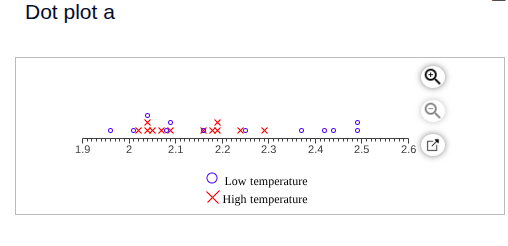
\includegraphics[width=\linewidth]{q1_dotplot_a.png}
  \caption*{\textbf{(a)}}
\end{minipage}\hfill
\begin{minipage}{0.48\textwidth}\centering
  
\includegraphics[width=\linewidth]{q1_dotplot_b.png}
  \caption*{\textbf{(b)}}
\end{minipage}

\vspace{0.6em}
\begin{minipage}{0.48\textwidth}\centering
  
\includegraphics[width=\linewidth]{q1_dotplot_c.png}
  \caption*{\textbf{(c)}}
\end{minipage}\hfill
\begin{minipage}{0.48\textwidth}\centering
  
\includegraphics[width=\linewidth]{q1_dotplot_d.png}
  \caption*{\textbf{(d)}}
\end{minipage}
\caption{The four candidate comparative dotplots.}
\end{figure}

\paragraph{Solution.}

\paragraph{Step 1: Sort each group.}
Ordering each row from smallest to largest makes the endpoints and clusters easy
to check against the plots:
\[
\begin{aligned}
\textbf{Low }(\SI{20}{\celsius}):\;
 & 2.02,\,2.04,\,2.04,\,2.05,\,2.07,\,2.09,\,2.16,\,2.18,\,2.19,\,2.19,\,2.24,\,2.29\\
\textbf{High }(\SI{45}{\celsius}):\;
 & 1.96,\,2.01,\,2.04,\,2.08,\,2.09,\,2.16,\,2.25,\,2.37,\,2.42,\,2.44,\,2.49,\,2.49
\end{aligned}
\]

\paragraph{Step 2: Identify ``fingerprint'' points that a correct plot must match.}
Rather than checking all $24$ marks, use the two extremes of the combined data
set --- they uniquely identify the correct plot:
\begin{itemize}[leftmargin=1.4em]
  \item \textbf{Overall minimum $=1.96$} belongs to the \emph{High} group, so the
        single left-most mark must be a \textcolor{red}{red $\times$}.
  \item \textbf{Overall maximum $=2.49$ (twice)} also belongs to the \emph{High}
        group, so the two right-most marks (stacked near $2.49$) must be
        \textcolor{red}{red $\times$}'s.
  \item The \emph{Low} group is tightly clustered: it never goes below $2.02$ or
        above $2.29$, so \textbf{no \textcolor{blue}{blue $\circ$} may appear at
        either extreme.}
\end{itemize}

\paragraph{Step 3: Test each option against the fingerprints.}
\begin{table}[h]
\centering
\renewcommand{\arraystretch}{1.3}
\begin{tabular}{c l l c}
\toprule
Plot & Left-most mark ($\approx1.96$) & Right-most marks ($\approx2.49$) & Verdict \\
\midrule
(a) & \textcolor{blue}{$\circ$} (blue)  & \textcolor{blue}{$\circ$} (blue)  & \ding{55}\ colors swapped \\
(b) & \textcolor{blue}{$\circ$} (blue)  & \textcolor{red}{$\times$} (red)   & \ding{55}\ min wrong color \\
(c) & \textcolor{red}{$\times$} (red)   & \textcolor{blue}{$\circ$} (blue)  & \ding{55}\ max wrong color \\
(d) & \textcolor{red}{$\times$} (red)   & \textcolor{red}{$\times$} (red)   & \checkmark\ matches data \\
\bottomrule
\end{tabular}
\caption{Only plot (d) places both extremes in the High-temperature group.}
\end{table}

Only \textbf{plot (d)} puts the smallest value \emph{and} the two largest values
in the High group, with the Low group confined to the $2.02$–$2.29$ band. It is
the only plot consistent with the data.

\begin{answerbox}
\textbf{Answer (a): Dot plot (d)} is the correct comparative dotplot.
\end{answerbox}

\subsection*{Part (b) — Sample mean tensile strength for each group}

\paragraph{Setup.} The sample mean is
\[
\bar{x}=\frac{1}{n}\sum_{i=1}^{n} x_i,\qquad n=12 \text{ for each group.}
\]

\paragraph{Low temperature (\SI{20}{\celsius}).}
\[
\sum x_i = 2.07+2.19+2.29+2.04+2.24+2.04+2.09+2.18+2.02+2.19+2.16+2.05 = 25.56,
\]
\[
\bar{x}_{\text{low}}=\frac{25.56}{12}=2.130\ \text{MPa}.
\]

\paragraph{High temperature (\SI{45}{\celsius}).}
\[
\sum x_i = 2.42+2.16+2.44+2.04+2.37+2.09+1.96+2.49+2.08+2.49+2.25+2.01 = 26.80,
\]
\[
\bar{x}_{\text{high}}=\frac{26.80}{12}=2.2333\ldots \approx 2.233\ \text{MPa}.
\]

\begin{answerbox}
\textbf{Answer (b):}\quad
$\bar{x}_{\text{low}} = 2.130$ megapascals \qquad
$\bar{x}_{\text{high}} = 2.233$ megapascals \quad(rounded to three decimals).
\end{answerbox}

\subsection*{Part (c) — Does curing temperature affect tensile strength?}

\noindent Based on the plot, choose the best statement and comment further:
\begin{enumerate}[label=\textbf{\Alph*.},leftmargin=2.2em,itemsep=2pt]
  \item Yes. The observations for the high-temperature group are generally
        \emph{lower} than the low-temperature group.
  \item Yes. The observations for the high-temperature group are generally
        \emph{higher} than the low-temperature group.
  \item No. The observations for the high-temperature group are similar to the
        low-temperature group.
  \item No. The plot cannot be used to distinguish between the two groups.
\end{enumerate}

\noindent
The high-temperature ($\SI{45}{\celsius}$) marks sit farther to the right than the
low-temperature ($\SI{20}{\celsius}$) marks: the high group has the larger center
($\bar{x}=2.233$ vs.\ $2.130$, median $2.205$ vs.\ $2.125$) and contains all of the
largest values ($2.37$–$2.49$). So curing temperature \emph{does} appear to affect
tensile strength, with higher temperature giving generally higher strength.

\begin{answerbox}
\textbf{Answer (c): B} --- Yes; the high-temperature observations are generally
higher than the low-temperature observations, so curing temperature appears to
increase tensile strength.
\end{answerbox}

\subsection*{Part (d) — Is anything else influenced by curing temperature?}

\noindent Choose the best statement and explain:
\begin{enumerate}[label=\textbf{\Alph*.},leftmargin=2.2em,itemsep=2pt]
  \item Yes. The high-temperature group also contains the lowest observations, so
        an increase in temperature leads to a \emph{decrease} in variability.
  \item Yes. The high-temperature group also contains the lowest observations, so
        an increase in temperature leads to an \emph{increase} in variability.
  \item No. The high-temperature group appears to have similar variability to the
        low-temperature group.
  \item No. The plot cannot be used to distinguish between the two groups.
\end{enumerate}

\noindent
Besides shifting the center up, the high-temperature ($\SI{45}{\celsius}$) group is
much more \emph{spread out}. It contains \emph{both} the smallest value in the whole
study ($1.96$) and the two largest ($2.49$), so its range is nearly double that of
the low-temperature group:
\[
R_{\text{high}} = 2.49 - 1.96 = 0.53
\quad>\quad
R_{\text{low}} = 2.29 - 2.02 = 0.27 .
\]
So a higher curing temperature appears to increase the \emph{variability}
(spread/consistency) of the tensile strength, not just its average.

\begin{answerbox}
\textbf{Answer (d): B} --- Yes; the high-temperature group also contains the lowest
observations, so an increase in curing temperature leads to an increase in
variability.
\end{answerbox}

\subsection*{Interpretation (what the plot and means tell us)}
The summary measures confirm what the dotplot shows:
\begin{center}
\renewcommand{\arraystretch}{1.25}
\begin{tabular}{l c c c c}
\toprule
Group & Mean & Median & Range & Spread \\
\midrule
Low (\SI{20}{\celsius})  & $2.130$ & $2.125$ & $0.27$ & tight cluster \\
High (\SI{45}{\celsius}) & $2.233$ & $2.205$ & $0.53$ & much wider \\
\bottomrule
\end{tabular}
\end{center}

\noindent
Raising the curing temperature from \SI{20}{}{} to \SI{45}{\celsius} shifts the
typical tensile strength \emph{up} (mean $2.130 \to 2.233$, median
$2.125 \to 2.205$) but also makes the results \emph{more variable} (range roughly
doubles, $0.27 \to 0.53$). So the higher curing temperature tends to produce
stronger --- but less consistent --- rubber, supporting the idea that tensile
strength is a function of curing temperature.

\subsection*{Reference}
Reading a \emph{comparative dotplot} and describing a distribution by its
\textbf{center} and \textbf{spread} are the Chapter~1 descriptive-statistics
ideas. The Chapter~1 lecture transcript develops the supporting numerical
measures used in the interpretation above: measures of center (mean, median,
mode) and measures of spread (range, variance, standard deviation).
\hfill{\small[\textit{Chapter1\_transcripts.txt}]}

%==============================================================================
% Add Question 2 here as \section{...} when ready.
%==============================================================================

\end{document}
